\documentclass[english, DIV=13]{scrreprt}

\usepackage[utf8x]{inputenc}
\usepackage[T1]{fontenc}
\usepackage{lmodern}
\usepackage{microtype}
\usepackage{xspace}
\usepackage[binary-units=true]{siunitx}
\usepackage{graphicx}
\usepackage{hyperref}
\usepackage{todonotes}
\usepackage{epstopdf}
\usepackage{array}
\usepackage{multicol}
\usepackage{multirow}
\usepackage{tabularx} % tabular with automatic line-break
\newcolumntype{Y}{>{\centering\arraybackslash}X} % centered column
\usepackage{amsmath}
\usepackage{grffile} % better name handling with graphicx
\usepackage{currfile} % provides relative file inclusion for tikzscale
\usepackage{listings}
\lstset{%
    basicstyle=\scriptsize\ttffamily,
    breaklines=true
}

\usepackage{tikz}
\usepackage{pgfplots}
\usepackage{pgfplots}
\usepackage{tikzscale}
\pgfplotsset{compat=newest}
\usetikzlibrary{plotmarks}
\usepackage{rotating}
\usepackage[absolute,overlay]{textpos}
\usepackage{circuitikz}

% Math symbols
\usepackage{amsmath}
\usepackage{amssymb}
\usepackage{amsthm}
\DeclareMathOperator*{\argmin}{arg\,min}
\DeclareMathOperator*{\argmax}{arg\,max}
\newcommand\norm[1]{\left\lVert#1\right\rVert}

% Sets
\newcommand{\Z}{\mathbb{Z}}
\newcommand{\R}{\mathbb{R}}
\newcommand{\Rn}{\R^n}
\newcommand{\Rnn}{\R^{n \times n}}
\newcommand{\C}{\mathbb{C}}
\newcommand{\K}{\mathbb{K}}
\newcommand{\Kn}{\K^n}
\newcommand{\Knn}{\K^{n \times n}}

% Unit vectors
\usepackage{esint}
\usepackage{esvect}
\newcommand{\kmath}{k}
\newcommand{\xunit}{\hat{\imath}}
\newcommand{\yunit}{\hat{\jmath}}
\newcommand{\zunit}{\hat{\kmath}}
\newcommand{\uunit}{\hat{\umath}}

% rot & div & grad & lap
\DeclareMathOperator{\newdiv}{div}
\newcommand{\divn}[1]{\nabla \cdot #1}
\newcommand{\rotn}[1]{\nabla \times #1}
\newcommand{\grad}[1]{\nabla #1}
\newcommand{\gradn}[1]{\nabla #1}
\newcommand{\lap}[1]{\nabla^2 #1}

% Elec
\newcommand{\B}{\vec B}
\newcommand{\E}{\vec E}
\newcommand{\EMF}{\mathcal{E}}
\newcommand{\perm}{\varepsilon} % permittivity

\newcommand{\bigoh}{\mathcal{O}}
\newcommand\eqdef{\triangleq}

\DeclareMathOperator{\newdiff}{d} % use \dif instead
\newcommand{\dif}{\newdiff\!}
\newcommand{\fpart}[2]{\frac{\partial #1}{\partial #2}}
\newcommand{\ffpart}[2]{\frac{\partial^2 #1}{\partial #2^2}}
\newcommand{\fdpart}[3]{\frac{\partial^2 #1}{\partial #2\partial #3}}
\newcommand{\fdif}[2]{\frac{\dif #1}{\dif #2}}
\newcommand{\ffdif}[2]{\frac{\dif^2 #1}{\dif #2^2}}
\newcommand{\constant}{\ensuremath{\mathrm{cst}}}


\title{LELEC2103}
\subtitle{Project in Electricity 3 : Electronic systems}
\author{Gaëtan Cassiers\and Antoine Paris}
\date{\today}

\begin{document}
\maketitle
\tableofcontents

\addchap{Introduction}
The objective of this project in electronic systems is to design and implement a
two-player video game using a Raspberry-Pi 3, a DE0-Nano board containing an FPGA
and a collection of interfaces and peripherals, and a multi-touch LCD display on
each side. In addition, the FPGA features a Nios II processor running µC/OS-II, a
real-time kernel.
One of the main specificity of this project is that each side is designed and
implemented by two independent groups. However, because the two players have to
communicate with
each other through a Wi-Fi communication between the two Raspberry-Pis, a common
network interface has been specified by the two groups. This is discussed
in chapter~\ref{chap:net-interface}. Before that, chapter~\ref{chap:gameplay-features}
introduces the game that inspired ours and the additional features we decided to
add to it. Section~\ref{chap:global-view} then describes the global architecture of
our game as a block diagram where each block, named subsystem in what follows, serves a
particular purpose. One of the key feature of our implementation of the game is the
3D rendering. Together with the frame compression system we designed, this really
constitutes the core of our project. These two subsystems are discussed in sections
\ref{sec:rendering} and~\ref{sec:compression} respectively.
To ensure robust and fast communication between the Raspberry-Pi and the FPGA, a smart
SPI slave subsystem together with a simple, yet reliable, communication protocol has
been designed and implemented. This is the topic of section~\ref{sec:spi}. Next, in
section~\ref{sec:display-mngt}, the hardware behind the double buffering technique
--- used to avoid tearing effects on the screen --- is explained.
In section~\ref{sec:input-det}, we head to the tasks running on the real-time kernel.
These tasks are responsible for the sensing of the touchscreen and the accelerometer.
Another originality of our game is that the players have the possibility to take a
selfie, either with a smartphone or a PC, to actually see themselves in the game.
Section~\ref{chap:pic-acq} explains this player pictures acquisition subsystem.

\chapter{Gameplay and features}
\label{chap:gameplay-features}

\section{Original game}
Our game is inspired by an existing game available on most smartphones and tablets
and developped by Ketchapp. Figure~\ref{fig:original-game} is a screenshot from this game.
In this original version of the game, the player (represented by the yellow cube on figure
~\ref{fig:original-game}) has to place itself correctly on the white structure in order
to fit in the hole of the wall coming in his direction at a constant speed. The objective
is to pass in as much wall as possible. Passing a wall gives 1 point, failing to pass a
wall makes the score starting back at 0.

\begin{figure}[bth]
    \centering
    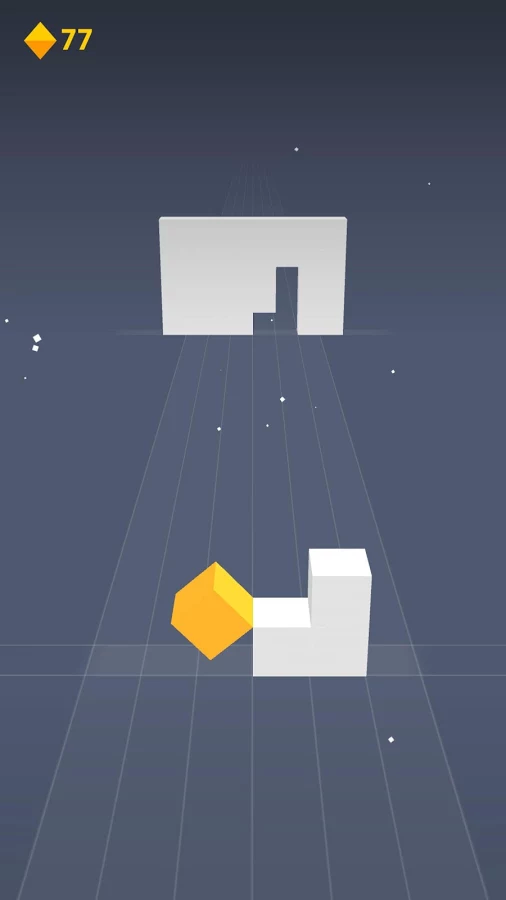
\includegraphics[width=0.3\textwidth]{img/original-game}
    \caption{Screenshot of the orginal game by Ketchapp.}
    \label{fig:original-game}
\end{figure}

\section{Custom version of the game}
Our version of the game differs from the original one in several aspects. First, this
is a collaborative game for two players. Second, a game only lasts a fixed amount of time
and the two players can control the speed of the wall using the accelerometer.
Finally, failing to pass a wall only decreases the current score by 1. 

\begin{figure}[bth]
    \centering
    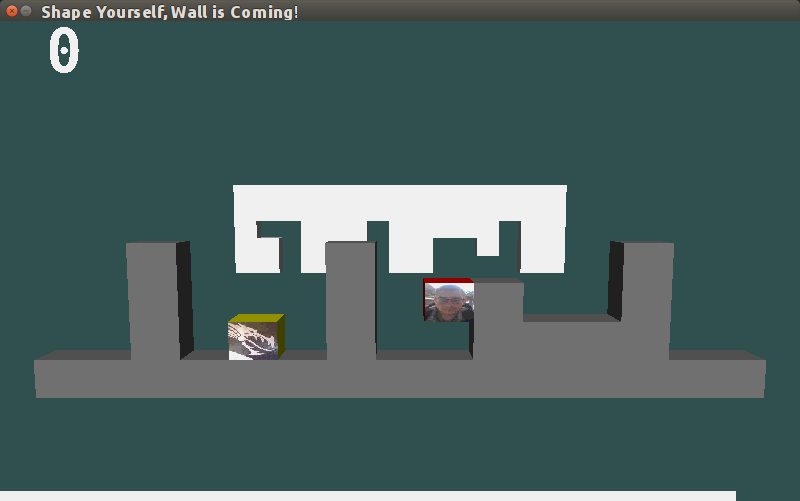
\includegraphics[width=0.7\textwidth]{img/custom-game-version}
    \caption{Screenshot of our version of the game. This screenshot has been taken
    on the PC version of the game but there is really no difference with the actual
    on-device version.}
    \label{fig:custom-game}
\end{figure}

\section{Additional features}
The difficulty of the game relies mainly on the fact that the scene is represented as a
3D image. Experience has shown that this can sometimes be really perturbating or even
induces the players in error. To counteract a bit this, and to add some fun to the
gameplay, the player can change de point of view of the 3D scene by tilting the tablet
on the left or on the right. In addition, the player has the possibility to make the
structure on which it stands disappear during a very small amount of time each round.
This feature can also help the player to better see where he should go to fit in the hole.

As briefly mentioned in the introduction, players also have the possibility to take a
selfie, either with a smartphone or a PC, to actually see themselves in the game. More
precisely, their picture appears on the cube they incarnate. In addition to beeing just a
cool feature, this helps the players to localize the cube they control at the start of
each round.

Finally, since playing our game requires a lot of concentration, players can pause the
game whenever they want to take a break.

To improve the advertising possibilities of the game, we also added a spectator mode,
by which a client (like a PC with a large screen) can display the scene shown to the
players whithout taking otherwise part in the game.

\chapter{Network interface}
\label{chap:net-interface}

The way the two players communicate with each other is illustrated in
figure~\ref{fig:comm-scheme}.
The approach taken here is client-server based. The server is responsible
for all the logic of the game and maintains an object representing the state of the game,
while the clients are simple input/output terminals that do no handle the logic of the
game. Centralizing computations in this way ensures an easy and robust synchronization
between clients.

\begin{figure}[hbt]
    \centering
    \includegraphics[width=0.8\textwidth]{img/global_comm_scheme_cropped.pdf}
    \caption{Block diagram of the network communication.}
    \label{fig:comm-scheme}
\end{figure}

A complete communication protocol was rigorously defined by the two groups (see full
protocol specification in appendix~\ref{app:protocol}).
This protocol defines an handshake procedure between a client and the server to ensure both
sides are ready before starting the game.
Once the game has started, the two clients can send
messages to the server based on user inputs (accelerometer values, touches, or gestures).
The server then performs some computations on the game state such as computing player
positions, speed and position of the wall, remaining time, score, etc. Finally, the server
broadcasts the parts of the game state which changed, and only those parts.

The protocol is designed to minimize the bandwidth used, which is achieved by using small packets
of a few bytes, that transfer only the part of the game state that changed.
This design makes the average bandwidth used less than \SI{1}{kb/s}.

All the communication happens over the TCP protocol. This protocol provides the reliability
layer. Its main drawback is to damatically increase the latency when there is a packet loss.
In our case this drawback is relatively minor since the latency and the packet loss rate
for point-to-point WiFi communication are small.

A spectator mode is defined: at any time of the game, a client can connect to the server,
advertising itself as a spectator and not as a player. The server then starts sending the
same information to the spectator as the one it sends to the players. The server ignores
any command coming from the spectator.

On the practical side, one Raspberry-Pi runs both the server and a client while the other
one only runs a client.
The Raspberry-Pi running the server is also configured as a WiFi access point and the other
Rapsberry-Pi is directly connected to it. This point-to-point setup maximizes the
reliability of the communication while minimizing the latency.

\chapter{Global view of the client system}
\label{chap:global-view}

The global view of the client system is represented in figure~\ref{fig:global-desktop}
and figure~\ref{fig:global-device}. Through the network interface described in the
previous chapter, the client builds its own image of the game state. This client game
state is then fed to the rendering subsystem which produces a 3D image. This image
is then compressed and sent to the hardware interface.

One of the strength of our system is this hardware interface. This abstraction offers
a common layer to communicate both with a PC or a device.
On PC, touches, gestures and accelerometer values are simulated with the keyboard.
This eased a lot the development process by allowing efficient debugging first on PC,
and then only on device if necessary.

On PC, the hardware interface mainly interacts with a Python library dedicated to game
developement named Pygame. As a first development step, Pygame allowed us to develop
a fully functionnal basic 2D version of the game. The move to the 3D version
complicated a lot the rendering subsystem. This is explained in
section~\ref{sec:rendering}.

\begin{figure}[bth]
    \centering
    \includegraphics[width=0.45\textwidth]{img/block_global_desktop_cropped.pdf}
    \caption{Block diagram of the client, when running on a PC.}
    \label{fig:global-desktop}
\end{figure}

On device, the hardware interface communicates through SPI with the FPGA.
Different types of informations flow in both directions. From the Raspberry-Pi to the
FPGA, compressed frames representing 3D scenes along with control signals for the
display manager are sent at a fixed rate. The reasons why we need a compression
subsystem between the rendering subsystem and the hardware interface are detailed in
section~\ref{sec:compression}. From the Nios processor running µC/OS-II, accelerometer
values and touchscreen events are periodically read out by the hardware interface.

\begin{figure}[bth]
    \centering
    \includegraphics[width=0.6\textwidth]{img/block_global_device_cropped.pdf}
    \caption{Block diagram of the client, when running the raspberry-pi/DE0-Nano system.}
    \label{fig:global-device}
\end{figure}

\section{Rendering subsystem}
\label{sec:rendering}

The rendering subsystem takes as input the state of the game sent by the server,
and outputs images of the size of the LCD screen at a rate
of 25 FPS. As shown in figure~\ref{fig:rendering}, the rendering system is
implemented as a pipeline and performs three main operations: draw instructions
computation, rendering of the 3D scene and blitting of text on top of the 3D scene.
Each of these operations is detailled below.

\begin{figure}[bth]
    \centering
    \includegraphics[width=0.5\textwidth]{img/block_rendering_cropped.pdf}
    \caption{Pipeline for the rendering of the video.}
    \label{fig:rendering}
\end{figure}

\subsection{Draw instructions}

This step of the pipeline is implemented using the Python programming language.
It converts the game state sent by the server into a set of properties for each
frame. The main computations here are:
\begin{itemize}
    \item Animation of the cubes rotation: knowing the previous and current
    position of each cube, as well as the time each cube moved, the rotation
    center and the rotation angle are computed.
    \item Wall distance extrapolation: to ensure smooth movement of the wall, its
    displayed position is extrapolated from the last position sent by the server
    and from the speed of the wall.
    \item Computation of the angle of view based on the accelerometer value.
    \item \todo[inline]{Anything else ?}
\end{itemize}

\subsection{3D rendering}

The draw instructions are then sent to a C++ code, which computes the rotation/translation
matrices for all elements of the scene. These matrices are then sent to the GPU of the
Raspberry-Pi.

The pictures of the players are received by the server in the JPEG file format.
They are then decompressed and copied to the RAM of the GPU as textures.

Once those parameters are set, the GPU then executes an OpenGL ES program to draw the
image. This program is the one that computes the perspective projection and the lightning
of the scene.
Finally, the resulting image is copied back into the CPU RAM.

\subsection{Text handling}

Text handling is made of three steps:
\begin{itemize}
    \item Font rasterization: the vector description of the glyphs (taken from a 
    \texttt{.ttf} file) are converted individually into a mask of pixels.
    \item Text rendering: the rasterized glyphs are copied next to each other according
    to a given text string. This produces a binary image mask, which indicates where
    the text pixels should be drawn.
    \item Text blitting: using the text offset position in the image, each pixel of the
    image corresponding to a pixel set to true in the mask is set at the color of the text.
\end{itemize}

\section{Compression subsystem}
\label{sec:compression}

\subsection{Objectives}

The need for a compression system comes from the following observation:
when transferring 25 frames of 800x480 pixels per second, with 12 bits per pixel,
the bandwidth needed is \SI{115}{Mb/s}. The memory needed for each frame
is \SI{600}{kB}.

In our system, the SPI bandwidth available to transfer the video is \SI{5}{Mb/s},
and the memory available on the FPGA (considering onchip memory only, the SDRAM
being used by the Nios/µC0S-II system) is \SI{30}{kB} per frame.

We thus need a compression by a factor larger than 20, that is such that
the video can be compressed in real-time. The decompression must be done
pixel per pixel, on-the-fly, since there is no memory available to store the
decompressed images.

\subsection{Principle}

\begin{figure}[bth]
    \centering
    \includegraphics[width=0.65\textwidth]{img/compression_scheme_cropped.pdf}
    \caption{Principle view of the compression scheme.}
    \label{fig:compression}
\end{figure}

The compression system is based on three steps (see fig.~\ref{fig:compression}):
the color quantization, the run-length coding, and the Huffman coding. The first
step is lossy, while the two other steps are lossless.

\paragraph{Color quantization} The precision for each color channel is
reduced to 4 bits. This step is a preprocessing step that makes it possible
to implement and improves the efficiency of the following steps.

\paragraph{Run-length coding} The image, represented as a list of pixels,
is converted to a list of pairs $(\text{color}, \text{number of repetitions})$.
The allowed sizes for the number of repetitions are
$1, 2, 3, ..., 16,$ $32, 64, ..., 4096$. This allows to encode most images with
a number of blocks that is not too far from the optimum, while keeping the set
of number of repetitions small, which is required for the Huffman compression.

\paragraph{Huffman coding} Two Huffman trees are built: one for the pixels colors
and one for the numbers of repetitions. Each element of the pairs generated
at the previous stage is encoded with the corresponding Huffman tree.
All the codewords are then concatenated together to form the compressed image.

\subsection{Impact of the color quantization}

The color quantization serves different purposes. For the run-length coding,
the quantization creates chunks of constant color when there is a
continuous shading. For the Huffman
coding, the reduction of the color depth from \SI{24}{bits/pixel} to
\SI{12}{bits/pixel} means the size of the colorspace is reduced from
\SI{16}{M} to \SI{4}{K}. This simplifies a lot the Huffman coding:
\begin{itemize}
    \item it is much easier to estimate the distribution of the colors
    to build the Huffman tree\footnote{The color and run-length distribution are
    estimated from a set of training images at compile time.};
    \item it keeps the codewords length small, which simplifies the implementation:
    the memory bandwidth required is smaller;
    \item it reduces the amount of logic gates required to implement a decoder,
    which makes it possible to fit it on the FPGA;
    \item it also makes the software encoder faster, for the same reasons
    (memory bandwidth, code size).
\end{itemize}

The color quantization has an impact on the quality of the images
but it is mainly visible on image area exhibiting a color gradient.
For these kinds of images,
it may introduce a "staircase" effect. To avoid this artefact to be visible,
the rendering process has been tuned to avoid producing color gradients
through the choice of an appropriate lightning scheme for the 3D scene (the lightning
has only the directionnal component of the phong lightning model).

\section{SPI slave subsystem}
\label{sec:spi}

In order to transmit the compressed images at the required rate, an efficient and
flexible SPI communication protocol is needed.
The one we were provided with has major issues for our application:
\begin{itemize}
    \item there is a fixed overhead of 8 bits per 32 payload bits transmitted,
    \item the chip select signal must be released between each transfer of 32 bits
    words, which is slow on the Raspberry-Pi side,
    \item the address to which the data is written is limited to 7 bits, which means
    the maximum memory size is 128 words (512 bytes).
\end{itemize}

We thus designed a new protocol that avoids these issues, but which keeps the same simple
function: accessing (read and write) to a RAM.
The core idea of this protocol is that it works in burst mode: after some configuration
steps,
only the payload bytes are transmitted in a whole sequence, whithout any interruption for
chip select release or control bits.

To implemente this idea, the protocol is based on the state machine shown in
figure~\ref{fig:spi}.
At the start a transfer, the state machine is in command state.
The master (i.e. the Raspberry-Pi) sets the base address of the client by
sending a control word. A second control word sets the state machine in reading or
writing state and configures the number of data words that will be read or written
(this is the burst lenght).
The words transmitted are read/written starting at the base address and then sequentially
in the next words of the memory.
Once the right amount of data words have been transmitted, the state machine returns to
command state.
All the data or control words are made of 32 bits. The base address and the burst length
are encoded on 28 bits, which allows for a \SI{1}{GB} RAM.

\begin{figure}[bth]
    \centering
    \includegraphics[width=0.37\textwidth]{img/spi_state_machine_cropped.pdf}
    \caption{State machine for the SPI communication protocol.}
    \label{fig:spi}
\end{figure}

The SPI slave that implements this protocol on the FPGA is connected to a SPI MMU module,
that presents three RAMs under the same address space to the Raspberry-Pi.
These RAMs are the interface of the image buffer of the display management system,
the \texttt{display control} buffer of the same system (see section~\ref{sec:display-mngt})
, and the RAMs used for communication between the Nios and the Raspberry-Pi.

\section{Display management}
\label{sec:display-mngt}

The system uses double buffering to avoid tearing in displayed images.
It is implemented by two RAMs on the FPGA (see fig.~\ref{fig:display-manager}).

The RAMs are connected to the decoder
(which decodes the code discussed in section~\ref{sec:compression})
through a multiplexer controlled by a \texttt{display control} register.

The RAMs are also connected to the SPI MMU. The write enable
signal of the RAMs are masked by the \texttt{display control} signal,
so that only the RAM that is not connected to the decoder is written.

The \texttt{display control} register can be read from the SPI MMU,
and can be written by the SPI MMU, but only through a buffer register,
in order for changes of \texttt{display control} to be synchronized
to the \texttt{end of frame} signal from the display controller.
This synchronization is again necessary to avoid tearing.

\begin{figure}[bth]
    \centering
    \includegraphics[width=0.81\textwidth]{img/display_manager_cropped.pdf}
    \caption{Block diagram of the display management and synchronization system.}
    \label{fig:display-manager}
\end{figure}

\section{Input detection subsystem}
\label{sec:input-det}

Three tasks runs on the real-time kernel µC/OSII. One of them is responsible
for sensing the touchscreen. It is implemented as a finite state machine periodically
refreshed at a sufficient rate to ensure responsiveness. The fact that the gesture
detection is implemented in software makes it really flexible. Three different types of
gestures are recognized by this task:
\begin{itemize}
    \item A simple touch with one finger: depending on the position where this touch
    occurs on the screen, this is interpreted as an instruction from the user to move
    its cube to the left or to the right;
    \item A vertical swipe with two fingers: this is the custom gesture we defined to
    pause or resume the game;
    \item A simple touch with three fingers: this custom gesture commands the
    disappearance of the stucture during a small amount of time (this feature is
    described in chapter~\ref{chap:gameplay-features}).
\end{itemize}
When one of this gesture is detected, the touch sensing task sends a particular
message to a second task through a message mailbox to inform it of which gesture
was detected. Upon reception of a message via its message mailbox, this second task
tries to acquire the mutex on the SPI RAM before writing a value corresponding
to the detected gesture at a particular address.

The last task periodically reads the accelerometer values and, after acquiring
the mutex , writes it in the SPI RAM. To avoid tremor on the change of point of
view of the 3D scene of game, which is controlled by one of the axis of the
accelerometer, a very basic low-pass filter is applied to the accelerometer
values upon receipt by the hardware interface.

The three tasks and the synchronization mechanisms they used are represented in
figure~\ref{fig:tasks-mc}.

\begin{figure}[bth]
    \centering
    \includegraphics[width=0.5\textwidth]{img/tasks_mC_cropped.pdf}
    \caption{Tasks and their relationships on the uC/OS-II operating system.}
    \label{fig:tasks-mc}
\end{figure}

\todo[inline]{Describe high-level communication protocol RPI<->nios over SPI}

\chapter{Player pictures acquisition}
\label{chap:pic-acq}

As mentionned in the introduction and in chapter~\ref{chap:gameplay-features},
one of the originality of our game is that it makes possible to actually see
a picture of you on the cube you incarnate. This feature is illustrated on
figure~\ref{fig:custom-game} where you can see Bilal playing with the famous
Terasic's dragon.

On a more technical side, figure~\ref{fig:pic-acq} describes how this actually
works. A very basic HTTP web server written in Python is running on the port 8080
of the Raspberry-Pi. When a user access through a web browser to the IP address
of the Raspberry-Pi on port 8080, the HTTP web servers serves a slightly modified
version of \textsc{JpegCamera}, an open-source JavaScript webcam image capture
library. The user can then take a picture, indicate which player he is and upload
the picture on the Raspberry-Pi at a pre-defined location. At the start of each new game,
the game server picks the two last uploaded images and sends it to the client so that

\begin{figure}[bth]
    \centering
    \includegraphics[width=0.5\textwidth]{img/block_pictures_cropped.pdf}
    \caption{Block diagram of the picture acquisition subsystem.}
    \label{fig:pic-acq}
\end{figure}

\addchap{Conclusion}

The result of all the careful design described above is a game application that
is playful and extremely robust. We review here the main design choices that
enables these characteristics.

While the game concept is relatively simple, it is not repetitive thanks to the
wide variety of structures that are automatically generated, and this automatic
generation is done with an algorithm that ensures that the resulting structure
always has playful properties. Furthermore, the players can adapt the
difficulty to their skills by changing the speed of the wall, so that the game
remains challenging as the players improve. The perspective view (3D rendering)
of the scene is indeed attracting at the first sight, and it also enables
advanced gameplay possibilities, namely: changing the point of view of the
player and making the structure and the players disappear. For the novice
players, the flexible rendering of text allows to easily give hints. Finally,
the flexible rendering system allows to use a PC insted of a
Raspberry-Pi-DE0-Nano-MTL system to play. Combined with the use of the spectator
mode on a large display, this gives a very efficient way to attract candidate players
during public demonstrations.

Robustness is a critical characteristic for a game. A way to achieve this is to
carefully test and debug all the code. This
was achieved through the extensive use of logs to be able to track down the
origin of each crash, even if it only appears sporadically. Nevertheless, the
design of the communication protocols and the different entities is also an
important point. Our approach at this level was to avoid as much as possible any
kind of state that is shared by two communicating entities, and that needs
bidirectionnal sychronization. Indeed, bidirectionnal synchronization logic is often
complicated and error-prone, so we prefer to avoid it. For the TCP
communication (which is itself a robust protocol), there are two distinct
states: the state of the game, which is computed by the server and sent to the
clients and the state of the clients which goes in the opposite direction. The SPI
communication is designed with the same principle: at a low level, the slave state
machine is controlled by the master (i.e. the Raspberry-Pi). At a higher level,
there are two infomation flows: the display information that comes from the
master, and the player actions that are sent by the slave. All this
communication does not require any form of handshake, which makes the impact of
the crash of any entity minimum: there is no full reset of both parts, the
communication is just interrupted until the entity restarts.

That being said, there are numerous possible improvements to the game. Apart
from all the addition of features to the gameplay, we want to highlight two
simple extensions that would make the game even more interesting. The first one
is the extrapolation of the player movement based on its inputs: currently, when
a player does some left/right action, the command is sent to the server, which
computes the new position of the player and sends it to the client. This means
that the feedback of the action of the player is delayed by one network
round-trip time (RTT). The client can predict the movement of the player to
avoids this round-trip delay. This feature would greatly improves the perceived
responsiveness of the game. However it would in some rare situations
(simultaneous movement of both players to the same position) cause small
glitches. The second feature extension is the possibility to have more than two
players. The network architecture already supports this, so only a few
changes in the codebase are required to make the game truly multiplayer.

\appendix

\chapter{Network specification}
\label{app:protocol}

\lstinputlisting{network-protocol.txt}

\end{document}

